\documentclass[12pt]{article}

\usepackage[utf8]{inputenc}
\usepackage[brazil]{babel}
\usepackage[a4paper,left=3cm, right=2cm,top=2.5cm, bottom=2.5cm]{geometry}
\usepackage{amsmath}
\usepackage{graphicx}
\usepackage{float}
\usepackage{multirow}
\usepackage{authblk}
\usepackage{fancyhdr}
\usepackage{xcolor}
\usepackage{cite}


\title{\textbf{ENG1456 - Algoritmos Genéticos - Trabalho 1}}
\author{\textbf{Aluno: Matheus Carneiro Nogueira - 1810764}}
\affil{}
\author{\textbf{Professora: Karla Figueiredo}}
\affil{}
\pagestyle{fancy}
\fancyhf{}
\lhead{{\small \textcolor{gray}{PUC-Rio ENG1456}}}
\renewcommand{\headrulewidth}{0pt}
\date{}
\renewcommand{\footrulewidth}{0pt}
\fancyfoot[C]{\thepage}

\begin{document}
	\maketitle
	\tableofcontents
	
	
	\begin{abstract}
		Este documento consiste no relatório do trabalho 1 do módulo de Algoritmos Genéticos da disciplina ENG1456 da PUC-Rio. O objetivo deste trabalho é estudar diferentes modelos de Algoritmos Genéticos para a tentativa de otimização da função $F6$ apresentada em sala. Foi utilizado o programa \textit{GADEMO} para gerar os modelos pedidos nos enunciados. Foram consultados os materiais de aula, o livro \cite{davis1991handbook} e outros materiais devidamente referenciados.
	\end{abstract}
	
\section{Reproduzindo Resultados}

\textbf{Enunciado:}
Variando os parâmetros, execute Algoritmos Genéticos de modo a obter resultados semelhantes aos apresentados no livro texto. Os parâmetros usados no livro se encontram na tabela abaixo. Compare as curvas referentes à média de 20 rodadas de cada GA.

Incluir dois gráficos: um com GA1-1, GA2-1 e GA2-2 e outro com GA 2 -3 e GA2-4.

Utilizar somente one-point-crossover.

\begin{figure}[H]
	\centering
	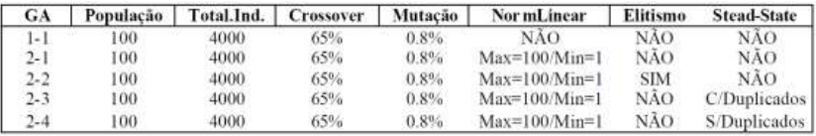
\includegraphics[width=0.9\linewidth]{Imagens/tabela_especificacao_modelos}
	\caption{Tabela com as especificações dos modelos}
	\label{fig:tabelaespecificacaomodelos}
\end{figure}

\section{GAP ideal}
Para os GAs que utilizam steady-state, determine o GAP (número de indivíduos substituídos a cada ciclo) ideal. Para isso, use um incremento de 5 indivíduos a cada tentativa, começando com um GAP=5. Não entregue os gráficos referentes aos testes de GAP.



	
\section{Taxas Crossover e Mutação}
\textbf{Enunciado:}
Verifique o que acontece quando se roda o GA2-1 20 vezes com taxa de crossover muito baixa (pouca recombinação em torno de 10\%) e alta taxa de mutação (muitas mudanças aleatórias em torno de 80\%). Imprima o resultado (um gráfico), compare com o resultado do GA2-1 obtido no item 1 e explique
brevemente o que acontece.

\section{Tamanho da População}
\textbf{Enunciado:}
Analise o efeito do tamanho da população, obtendo as curvas de desempenho do GA2-2 (20 rodadas) para vários tamanhos de população (ex: 20, 50, 100, 150) e sempre com o mesmo número de gerações (total de indivíduos variável). Imprima as curvas para e tire conclusões sobre o efeito do tamanho da população no desempenho do
algoritmo genético.

\section{Convergência}
\textbf{Enunciado:}
Repita o GA2-1 e o GA2-2 (20 rodadas cada) modificando apenas o total de indivíduos criados para o 10000. Imprima as curvas em dois um gráficos separados, um para o GA2-1 e outro para o GA2-2, e verifique se é vantajoso todo esse esforço computacional, em outras palavras, determine o número de
indivíduos para o qual cada algoritmo converge.

\section{Crossover}
\textbf{Enunciado:}
Compare o efeito dos 3 tipos de crossover disponíveis na ferramenta, executando o GA2-1 (s/ elitismo) e o GA2-2 (c/elitismo) com apenas 2500 indivíduos (20 rodadas) para cada tipo de crossover, usando taxa de crossover 80\%. Imprima as curvas em dois um gráficos separados , um para o GA2-1 e outro para o GA2-2, e tire conclusões a respeito da característica conservadora/destrutiva de cada crossover.


\section{Normalização Linear}
\textbf{Enunciado:}
Repita o GA2-3COM gap = 75 para vários valores de máximo. Verifique o que acontece quando o valor de máximo aumenta e diminui (avalie para os valores 10, 50, 100, 200, 300). Imprima as curvas em apenas um gráfico e tire breves conclusões .

\section{Gerais}
\textbf{Enunciado:}
Fazendo variações nos parâmetros e técnicas disponíveis no GADEMO, estude livremente o efeito de cada umdestes no desempenho de algoritmos genéticos. Destaque e explique uma importante constatação.

	\bibliography{bibliografia} 
	\bibliographystyle{plain}
\end{document}